In this chapter, we discuss how we managed the project. We will cover the software development 
methodology we used, the various stages of the project and how it relates to our timeline.
\section{Software Development Methodology}
We use an agile software development methodology to manage the project. Specifically, we use 
a combination of Scrum and Kanban to manage our sprints and features. Moreover, we adopt 
Test Driven Development (TDD) to ensure that we have a thorough and robust verification 
workflow to ensure the correctness of our code. 

We chose an agile software development 
methodology because there was a significant knowledge gap regarding the background material 
at the start of the project. As a result, it was difficult to accurately estimate the 
complexity of tasks and the time required to complete them. In the case that research and 
learning takes longer than expected, we would have to re-prioritise our tasks and change 
the scope of the project. 
Agile software development methodologies are well suited for this type of project because 
they allow for rapid iteration and adaptation to changing requirements. This actually 
proved useful in the later half of the project when issues with the code took longer to 
resolve than expected, causing delays. When this happened, we decided to prioritise 
the implementation of features and benchmarks and moved the implementation of security 
tests to the backlog. Even though this neglects and important aspect of cryptographic 
systems, it was necessary to ensure that we could complete the main objective of the 
project in time.

\subsection{Test Driven Development}
To prioritise functionality and validate that our features meet the requirements of the protocols, 
we use Test-Driven-Development (TDD) in our software 
development process. TDD is a programming style where tests are written 
based on requirements before features that aim to pass these tests are 
implemented. We show an illustration of the TDD software development 
lifecycle in Figure \ref{fig:tdd} below.

\begin{figure}[h]
    \centering
    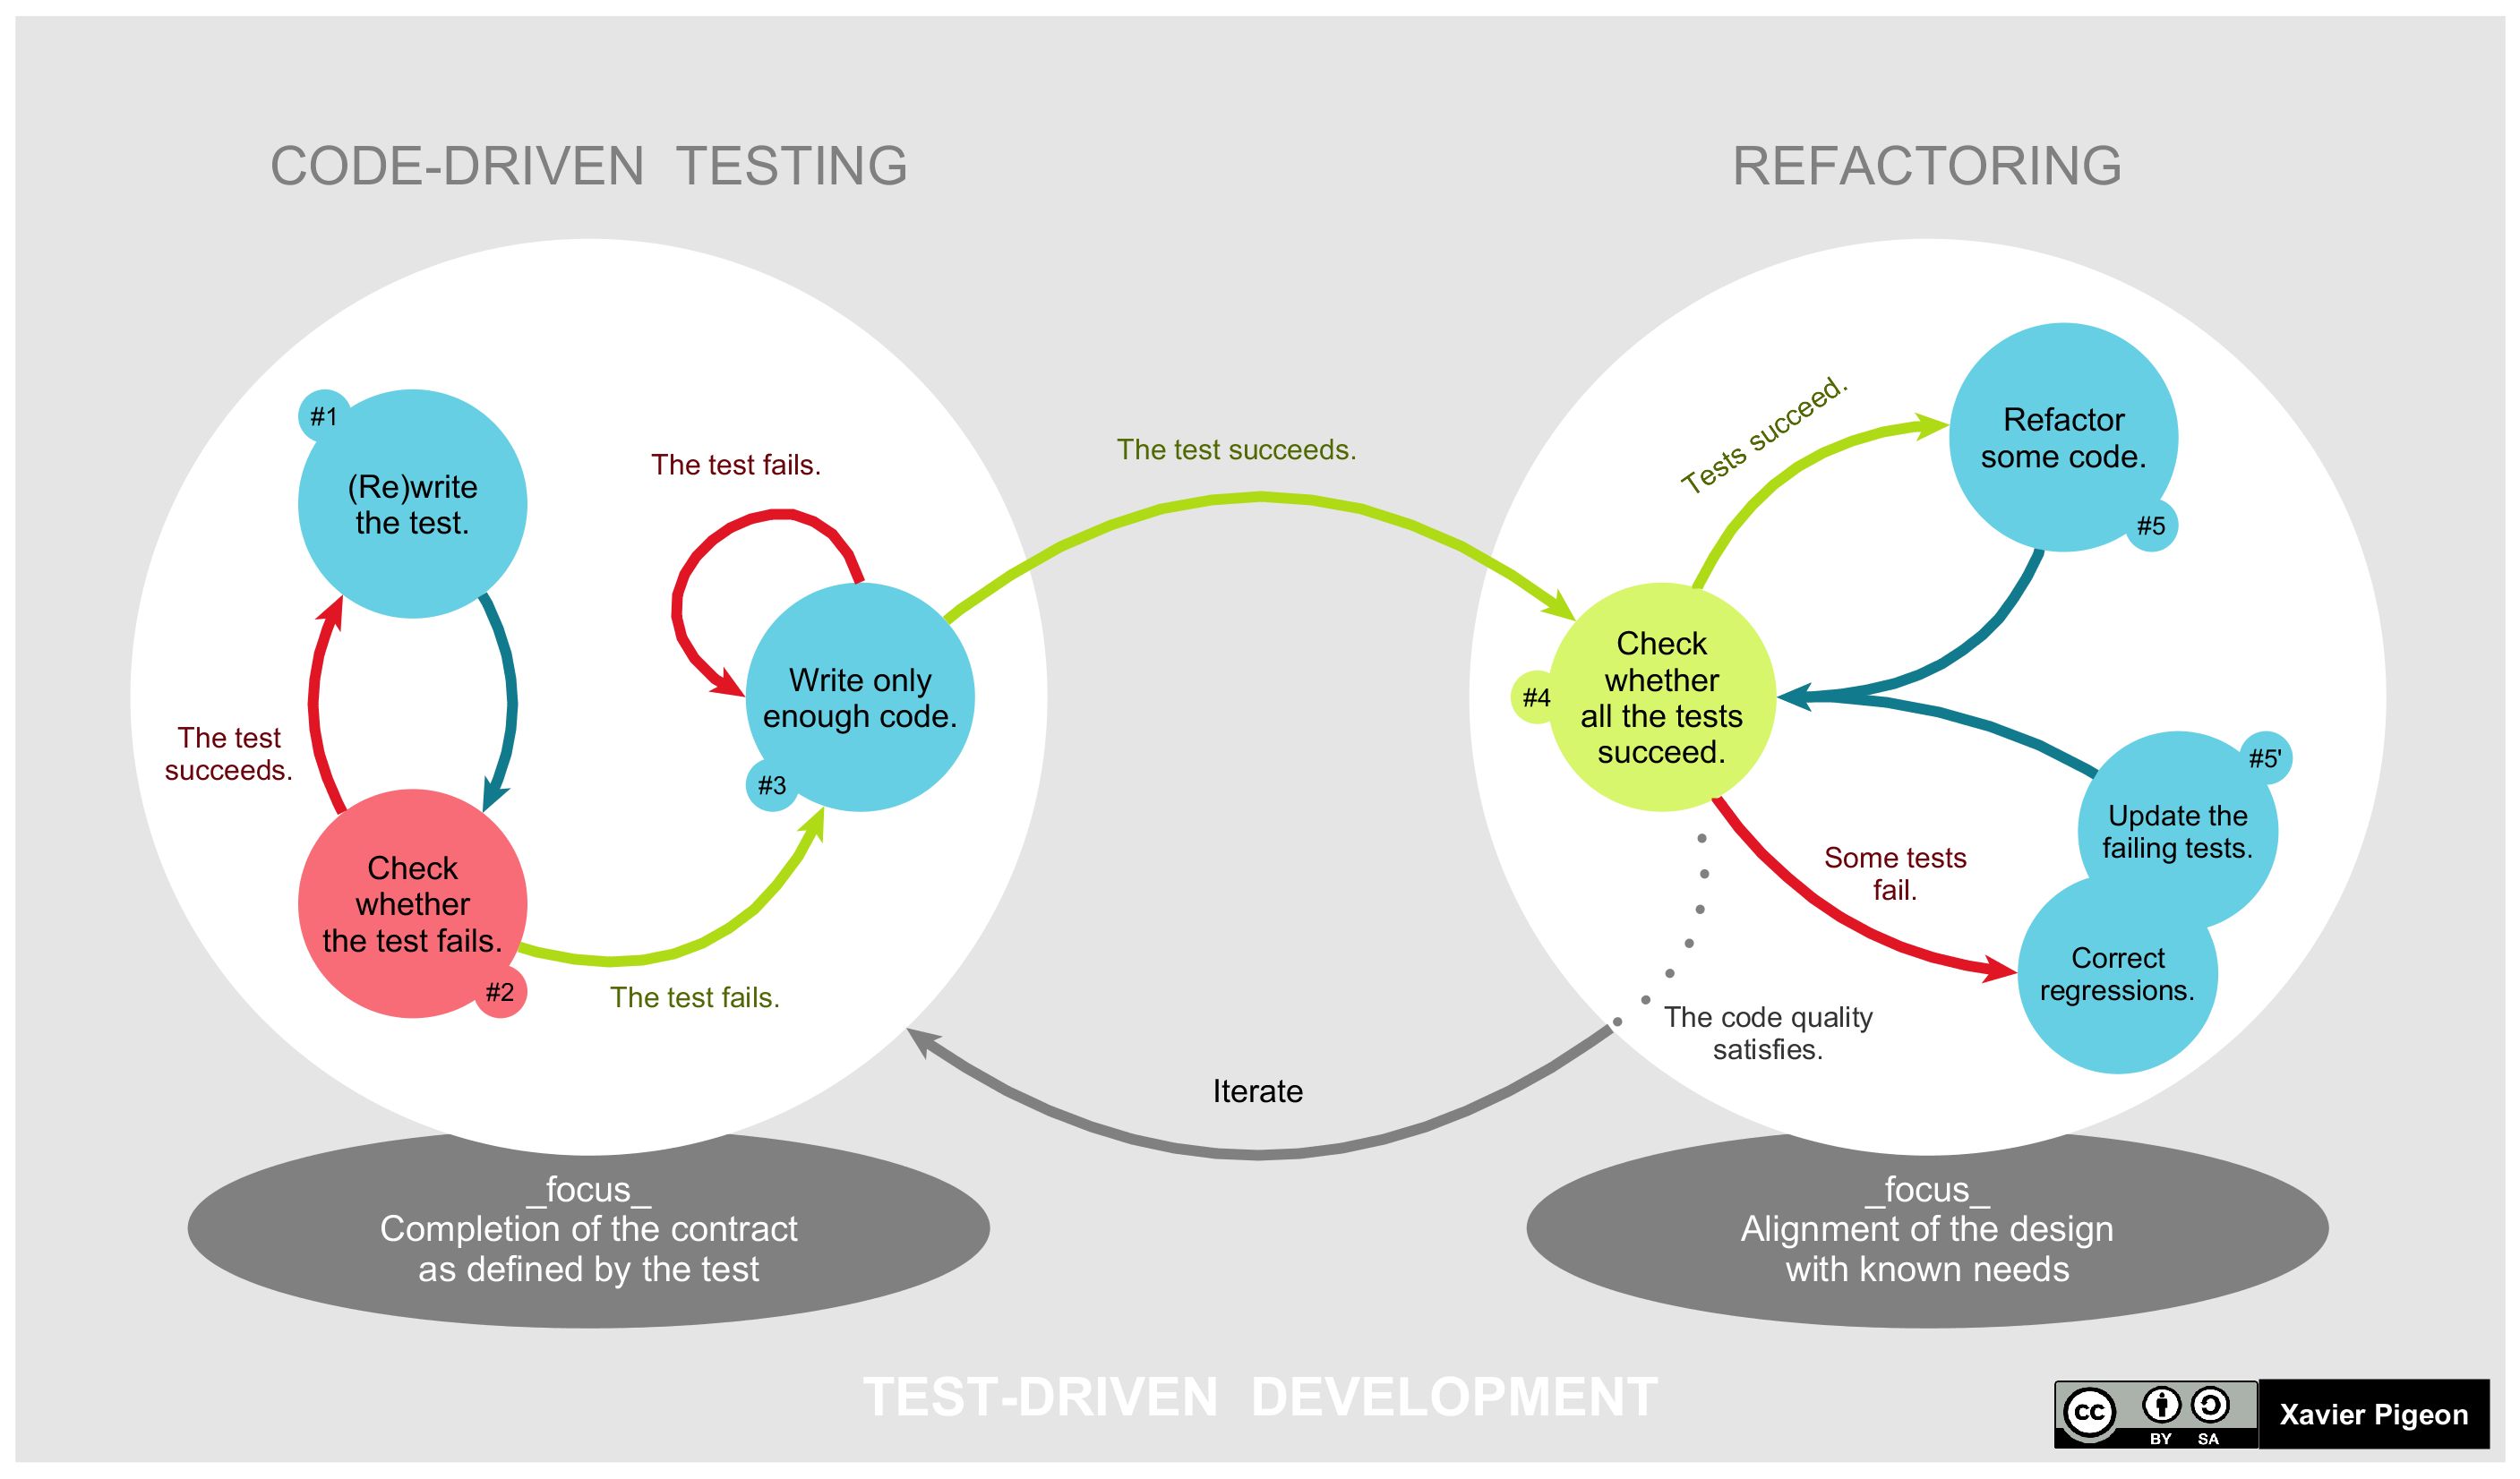
\includegraphics[width=\linewidth]{../assets/TDD_Global_Lifecycle.png}
    \caption{TDD Lifecycle \cite{Wikimedia:TDD}}
    \label{fig:tdd}
\end{figure}

TDD places an emphasis on first producing code that is minimally sufficient 
to pass the written tests. After which, code is refactored until it 
fulfils standard best practices such as readability, modularity, 
encapsulation etcetera. This appropriately prioritises functionality over 
readability, but still upholds written code to a high quality of design. 
This is especially so for this project as we prioritize correctness to 
ensure that we are providing meaningful results in our benchmarks.

Writing tests before implementation also helps during regression testing, to identify bugs 
when changes are made. This will not only improve code quality, but also make development 
more efficient. 


\subsection{Scrum and Kanban} Scrum is an agile project management framework that emphasises on 
flexibility and continuous improvement of software \cite{scrumguide}. 
It breaks down the development of a project 
into short iterations called sprints, which in our case are 2 weeks long. Meanwhile, Kanban is a 
another project management framework that share similar principles to Scrum and is often used 
in synergy with Scrum \cite{kanbanscrum}. Kanban focusses on visualising the workflow and 
limiting the number of features being worked on at any one time. This is done using a Kanban 
board, which is a visual representation of the tasks in the backlog, their current status, and 
the overall workflow. 
By controlling the number of features being worked on, 
it ensures that we complete features in a timely manner and do not run the risk of multitasking 
and causing delays. 

In this project, we use Kanban to manage our features and Scrums to manage development 
of said features. We use the Kanban board provided by Github to track all 
the features that we have planned for the project.
\begin{enumerate}
  \item Features are first added to the project backlog and then moved when the next sprint is
  planned. Features may be added to the backlog during development if need be, providing 
  flexibility while keeping the current sprint manageable. 
  \item At the start of each sprint, we plan the group of features to work on 
  for the next 2 weeks, and move them to the "To-do" column of the Kanban board. This column 
  is also known as the "Sprint Backlog".
  \item During the sprint, we move the features to the "Write Tests" column when we start writing 
  tests for the feature, based on the requirements.
  \item Once the tests are written, we start with the implementation and 
  move the feature to the "Implement" column. Throughout the implementation phase, we regularly 
  run tests to verify that the code is working as expected. We first focus on implementing 
  a minimally functioning feature, and testing for correctness. After which, features are 
  refactored to be more optimal if time allows for it. Tests may be refactored or added 
  when necessary to be consistent with the updated code or requirements.
  \item Once the feature is 
  fully tested and verified to be working, we move it to the "Done" column, indicating that 
  it is ready to be merged into our main branch. 
  \item At the end of the sprint, we review the features that were completed and ensure that 
  the project is on track with the timeline. We also plan the next sprint, repeating the cycle 
  again. Any additional features that were added to the backlog during implementation are 
  usually added during this planning phase to the next sprint.
\end{enumerate} 

To summarise, we use Kanban as a visualisation tool and to control the features in progress, Scrum 
is used to manage the development of these features in sprints. Finally, TDD is used to ensure 
that the code is correct and that the features meet the requirements. 

\section{Timeline}
We split the project into 3 main stages: research and learning, development of CDS94, and 
development of Stacking Sigmas. The two development stages also include benchmarking the 
respective compilers and anlaysing the data collected. We did not create a separate stage 
for the benchmarks because they were best done in parallel with the development of the
compilers.
In Table \ref{table:timetable_final}, we show the overall timeline of the project. In the "Goal" 
column, we indicate with a checkmark if the goal was achieved. Comments are provided in 
brackets where relevant. 

\begin{table}
  \centering
  \caption{Overall Project Plan}
  \begin{tabular}{p{0.2\linewidth}p{0.45\linewidth}p{0.25\linewidth}}
  \toprule
  \bf Sprint & \bf Main Task & \bf Goal \\ 
  \midrule
  T1 W1-2
  & Conduct necessary background reading and research.
  & Submit project specification. \checkmark
  \\\addlinespace[\rowheight]
  T1 W3-4
  & Understand the literature and extract requirements from the design of CDS94.
  & Must be capable of explaining CDS94 protocol to project supervisor. \checkmark
  \\\addlinespace[\rowheight]
  T1 W5-6
  & Familiarise with Rust and research libraries to use for implementation.
  & Finalise features to develop for CDS94 \checkmark
  \\\addlinespace[\rowheight]
  0 (T1 W7-8)
  & Begin implementation of CDS94.
  & Submit progress report. \checkmark
  \\\addlinespace[\rowheight]
  1 (T1 W9-10)
  & Implementing CDS94.
  & - (Completed goal in the next sprint early)
  \\\addlinespace[\rowheight]
  2 (Christmas Break)
  & Continue work on CDS94. 
  Start implement benchmarks. 
  Study and research \cite{StackingSigmas}.
  & \sout{Complete CDS94 }
  \\\addlinespace[\rowheight]
  3 (T2 W1-2)
  & Benchmark tests for CDS94 and collect data. Begin implementation of 
  Stacking Sigmas.
  & Complete benchmarks for CDS94. \checkmark
  \\\addlinespace[\rowheight]
  4 (T2 W3-4)
  & Implementing Stacking Sigmas. Update benchmark tests if necessary.
  & Complete implementation of Stacking Sigmas. (Delayed: 1 sprint)
  \\\addlinespace[\rowheight]
  5 (T2 W5-6)
  & Implementing Stacking Sigmas. 
  Benchmark Stacking Sigmas compiler and organise data collected for final presentation. 
  & Able to explain concepts in \cite{SpeedStacking} to project supervisor. (Delayed: 1 sprint)
  \\\addlinespace[\rowheight]
  6 (T2 W7-8)
  & Preparation for final presentation. Attempt basic implementation of Speed Stacking.
  & Present data to supervisor before presentation \checkmark
  \\\addlinespace[\rowheight]
  7 (T2 W9-10)
  & Continue with Speed Stacking.
  & Final Presentation. \checkmark
  \\\addlinespace[\rowheight]
  Easter Break
  & Write up of final report alongside exam revision.
  & Submit first draft of report for review (\checkmark).
  Complete Speed Stacking (No longer possible).
  \\\addlinespace[\rowheight]
  T3 W1-2
  & Final proof reading and editing of report.
  & Submit final report. \\
  \bottomrule
  \end{tabular}
  \label{table:timetable_final}
\end{table}


\paragraph{Research and Learning.} In the first stage of the project (6 weeks), time was dedicated 
to learning any background material and to study the literature. 
This was also the time when we familiarised ourselves with the programming language of choice: Rust. 
Tools and libraries that ended up being helpful to us in the project were also discovered during 
this period, through research and experimentation. It was imperative that we spent this time 
understanding the literature, as it would otherwise be difficult to implement the protocols accurately.
To ensure that we were ready to start development, we organised meetings with the 
project supervisor dedicated to clarifying details on the research material and to validate 
our understanding of the background material as a whole.  

\paragraph{Development.} The second and third stages (18 weeks) are similar in that they are 
dedicated to the development of the project. Yet, we decided to separate them into 2 stages as 
we anticipated that the time taken for the first stage (research) may be longer than 
we expect. In this scenario, we would be able to quickly re-prioritise and change the scope of 
the project if necessary. Fortunately, this was not the case and we were able to complete 
our initial objectives in time. 

This development phase is split into sprints: each of 2 weeks, except during the Christmas break 
where it was extended to 4 weeks. The CDS94 compiler was completed in the first 2 sprints, 
which surpassed our expectations. However, this did not include the implementation of the 
benchmarks and benchmarking CDS94. The benchmarks were completed over the next 2 sprints 
before work on 
the Stacking Sigmas compiler began. Unforunately, this took longer than expected due to the 
complexity of 
implementing the partially-binding vector commitment scheme. Furthermore, 
issues with the code were discovered during testing, which took an entire sprint to solve. 
During this period, we decided to not prioritise security testing on our compilers, and focus 
on correctness and collecting data from the benchmarks instead. In the end, development and 
benchmarking of Stacking Sigmas required 3 sprints, which is longer than expected but still within 
the time frame of the project. 

We also mentioned the possibility of implementing the 
Speed Stacking compiler \cite{SpeedStacking} in the project specification, and started work on 
it, but ultimately are not able to complete it in time for this report. That said, we still 
deem the project a success as we were able to complete the CDS94 and Stacking Sigmas compilers 
and collect insightful data from the benchmarks. 

\section{Project Management Tools}
We use Github to manage our entire project. Github is a web-based hosting service for version 
control using Git, and it also provides project management tools. Notably, it provides a 
Kanban board with "Github Projects" and sprint management with "Github Milestones". We manage 
features using the Kanban board, creating drafts when we are planning and converting these 
features into "Github Issues" when we are ready to start development. This automatically creates a 
Git branch for the feature, which we can work on and subsequently merge into our main branch 
when the feature is complete. 

\section{Risk Management}
Below we list the risks that we identified at the start of the project and how we mitigated
challenges that arose during development.
\begin{itemize}
  \item \textbf{Lack of experience.} We were not familiar with the Rust programming
  language or the background material initially and planned the project with this in mind. This 
  is why we dedicated the first 6 weeks to learning the language and the literature. Additionally,
  to prepare for the case that this phase would take longer than expected, we opted for an agile 
  development methodology to remain adaptive to changes in the project scope if necessary.
  \item \textbf{Unexpected challenges.} To prepare for unexpected delays in development, we 
  planned the project with a clear priority of the requirements: correctness firstly, then 
  usability and generality, followed by performance and security. This allowed us to focus on
  the most important aspects of the project first, and to prioritise the remaining features
  accordingly. Splitting the development of the two compilers into separate stages also allowed 
  for the possibility of changing the scope to focus on solely CDS94 if necessary. 
  \item \textbf{Machine Failure.} We used proper version control practices with the aid of 
  Git and Github to ensure that work can continue even if a machine fails. We also verified 
  that our programming tools were compatible with the university machines. This came in useful 
  when we had to switch to a different machine due to a hardware failure.
  \item \textbf{License Agreements.} The project relies on many existing libraries for 
  cryptographic primitives and other utilities. We ensured that the licenses of these libraries
  were compatible with our project. 
\end{itemize}
